\documentclass{article}

% Language setting
% Replace `english' with e.g. `spanish' to change the document language
\usepackage[english]{babel}

% Set page size and margins
% Replace `letterpaper' with`a4paper' for UK/EU standard size
\usepackage[letterpaper,top=2cm,bottom=2cm,left=2cm,right=2cm,marginparwidth=1.75cm]{geometry}

% Useful packages
\usepackage{amsmath}
\usepackage{graphicx} % for images
\usepackage{listings}
\usepackage[colorlinks=true, allcolors=blue]{hyperref}
\usepackage{url}
\usepackage{fancyhdr}
\usepackage[most]{tcolorbox}
\usepackage{minted}

% Hyperlink Customization
\usepackage{hyperref}
\definecolor{imperialBlue}{RGB}{0, 60, 120}
 \hypersetup{
     colorlinks=true,
     linkcolor=imperialBlue,
     filecolor=blue,
     citecolor = black,      
     urlcolor=imperialBlue,
     }


% Custom boxes
\newtcolorbox{blackbox}[1][]{colframe=black,colback=white,sharp corners,center,#1}

% Source Code
\definecolor{commentsColor}{rgb}{0.497495, 0.497587, 0.497464}
\definecolor{keywordsColor}{rgb}{0.000000, 0.000000, 0.635294}
\definecolor{stringColor}{rgb}{0.558215, 0.000000, 0.135316}
\lstset{ %
  backgroundcolor=\color{white},   % choose the background color; you must add \usepackage{color} or \usepackage{xcolor}
  basicstyle=\footnotesize,        % the size of the fonts that are used for the code
  breakatwhitespace=false,         % sets if automatic breaks should only happen at whitespace
  breaklines=true,                 % sets automatic line breaking
  captionpos=b,                    % sets the caption-position to bottom
  commentstyle=\color{commentsColor}\textit,    % comment style
  deletekeywords={...},            % if you want to delete keywords from the given language
  escapeinside={\%*}{*)},          % if you want to add LaTeX within your code
  extendedchars=true,              % lets you use non-ASCII characters; for 8-bits encodings only, does not work with UTF-8
  keepspaces=true,                 % keeps spaces in text, useful for keeping indentation of code (possibly needs columns=flexible)
  keywordstyle=\color{imperialBlue}\bfseries,       % keyword style
  language=C,                 % the language of the code (can be overrided per snippet)
  otherkeywords={*,...},           % if you want to add more keywords to the set
  numbers=left,                    % where to put the line-numbers; possible values are (none, left, right)
  numbersep=5pt,                   % how far the line-numbers are from the code
  numberstyle=\color{commentsColor}, % the style that is used for the line-numbers
  showspaces=false,                % show spaces everywhere adding particular underscores; it overrides 'showstringspaces'
  showstringspaces=false,          % underline spaces within strings only
  showtabs=false,                  % show tabs within strings adding particular underscores
  stepnumber=1,                    % the step between two line-numbers. If it's 1, each line will be numbered
  stringstyle=\color{stringColor}, % string literal style
  tabsize=2,	                   % sets default tabsize to 2 spaces
  title=\lstname,                  % show the filename of files included with \lstinputlisting; also try caption instead of title
  columns=fixed                    % Using fixed column width (for e.g. nice alignment)
}

\pagestyle{fancy}
\fancyhead[R]{\leftmark}
\fancyhead[L]{C GROUP PROJECT FINAL REPORT}
%\renewcommand{\headrulewidth}{0pt}
\fancypagestyle{firstpage}{%
  \lhead{ 
\includegraphics[width=3cm]{Imperial-College-logo.png} }
  \rhead{ 
\includegraphics[width=0.7cm]{C_logo.png}}
}

% Font Family
\renewcommand{\familydefault}{\sfdefault}
% No weird indentation
\setlength{\parindent}{0pt}
% \lstset{basicstyle=\ttfamily}

\title{C Group Project Final Report}
\author{Naman Sharma, Karim Selih, Panayiotis Gavriil and Konstantinos Koupepas}

\begin{document}
%
\includegraphics[scale=0.1]{Imperial-College-logo.png}
\maketitle
\thispagestyle{firstpage} 
\tableofcontents


\section{Assembler: Structure and Implementation}
\rule{\textwidth}{0.05em}
\vspace{0.1em}

For our implementation of the assembler, we chose to go with the two-pass assembly method and create a symbol table in the form of a hash table. Similar to the emulator, we broke down the task into the 4 main instruction types, the tokenizer and the general assemble/output functions. Together, we planned the header files and the tokenizer so that we would know how to receive the mnemonics, opcodes and operands of an instruction. Figure 1 shows how we organised our project - using header files. \\  \par \noindent
We allocated team members to complete these sub-tasks. Panayiotis was responsible for creating the hash table and the output/binary writer. Naman wrote the single data transfer function. Karim oversaw the tokenizer and the main assemble function.  Konstantinos wrote the branch, multiply and data processing functions. \\  \par \noindent
In general, assemble would read in the program instructions and perform two passes in order to create the hash table and then pass each instruction to its corresponding binary translation function. The tokenizer would parse the instruction into a structure based on which of the four types of instructions would generate the necessary binary encoding. \\  \par \noindent
One of the toughest aspects of implementing the assembler was to determine how to pass the operands to each of the four instruction types, since each instruction type had a different syntax and varying number of operands. We opted to use a structure which would clarify, for the specific opcode mnemonic, how many operands there would be and provide these operands as an array in the same order as provided in the spec's given syntax. \\ \par \noindent
Moreover, implementing a Hash Table in C was quite challenging but fun. The idea is simple, each of the entries contains a key and a value, a hashing algorithm (in our case that was the djb2 hashing algorithm) is applied to the key to determine the index of the value that is to be stored in the array. This becomes interesting when the result of the hashing algorithm is the same for two, or more, keys. Then, we say that a collision has occurred and a, so-called, overflow bucket has to be created. For this reason we decided to also implement the Linked List data structure so that when a collision occurs we can "chain" such a list to the key that caused the collision and store the values whose keys collided in it. Searching for a value in the table is simple, just pass its key to the hashing function to get the index where it should be and in case of reaching a bucket, iterate through the list until you find the value whose key exactly matches with the provided one. To delete a value, search in the table using its key and reset the entry where that key is found, and in the case of stumbling upon a bucket, make sure to change the pointer of the previous node to not point to the deleted entry but to the entry after that. \\ \par \noindent

\begin{blackbox}
\begin{lstlisting}[basicstyle=\large,language=C]
typedef struct
{
    enum Mnemonic mnemonic;
    int num_operand;
    char **operands;
} tokens_t;
\end{lstlisting}
\end{blackbox}

\begin{figure}[!ht]
\centering
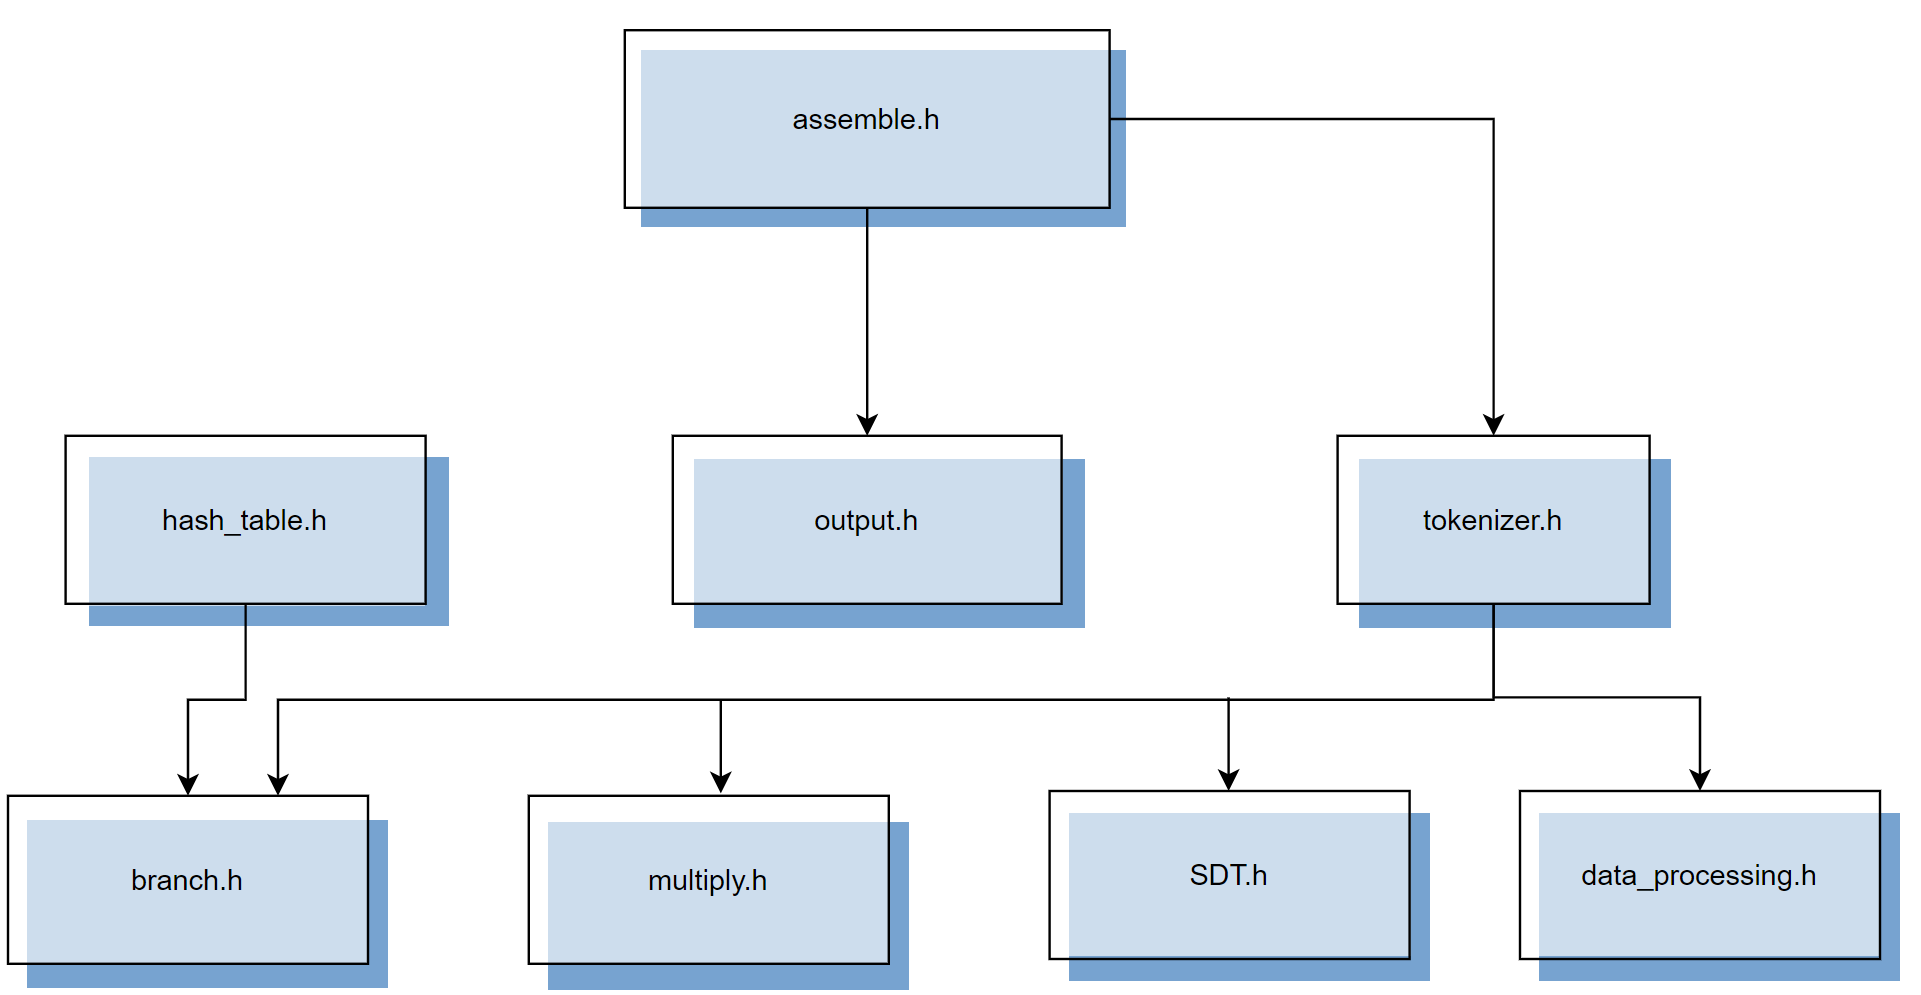
\includegraphics[scale=0.7]{AssemblerStructureStylized.png}
\caption{A layout of the assembler's headers files and their inter-dependencies.} 
\end{figure}

\clearpage

\section{Extension: Pac-Man}
\rule{\textwidth}{0.05em}
\vspace{0.1em}

\subsection{Description}
For the extension, we decided to recreate Pac-Man which we all used to play as children, since we thought it would be a fun exercise and good experience to create a game (which was the first time for many of us).  \\  \par \noindent
We ensured to read the original 1980 game specification on the Pac-Man wiki so that we could implement the game correctly. Specifically, when implementing the different targeting for the ghosts Inky, Blinky, Pinky and Clyde. This ensured that the ghosts would not move randomly or to the same target, but try to corner Pac-Man (apart from Clyde who gets scared).


\begin{figure}[h!]
\centering
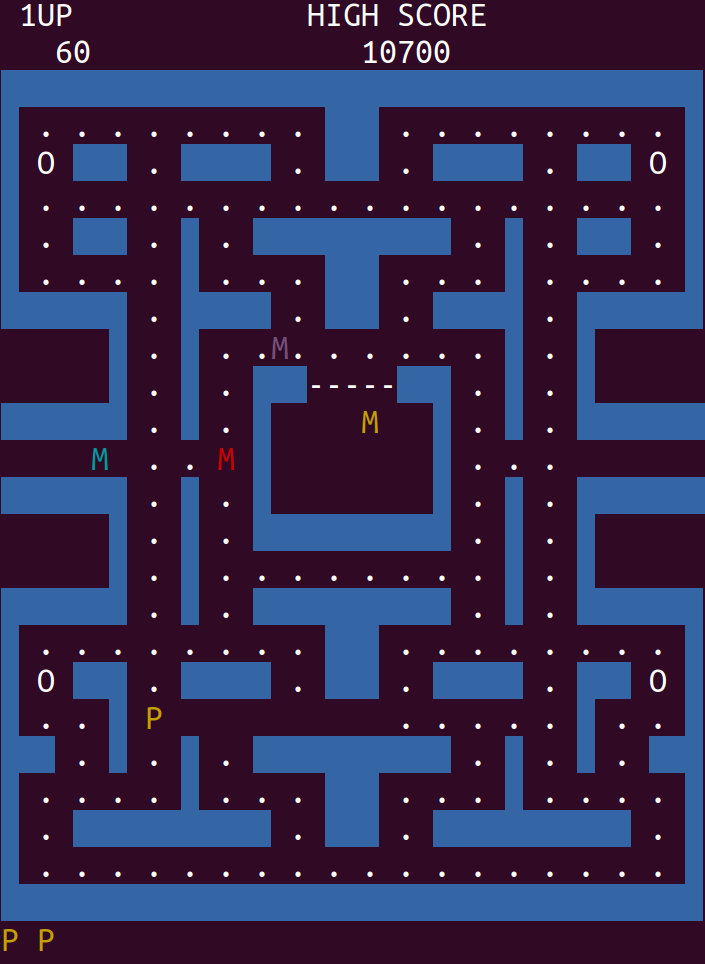
\includegraphics[scale=0.4]{pacman.PNG}
\caption{Our version of Pac-Man}
\end{figure}

\clearpage


\subsection{Design}
\begin{figure}[h!]
\centering
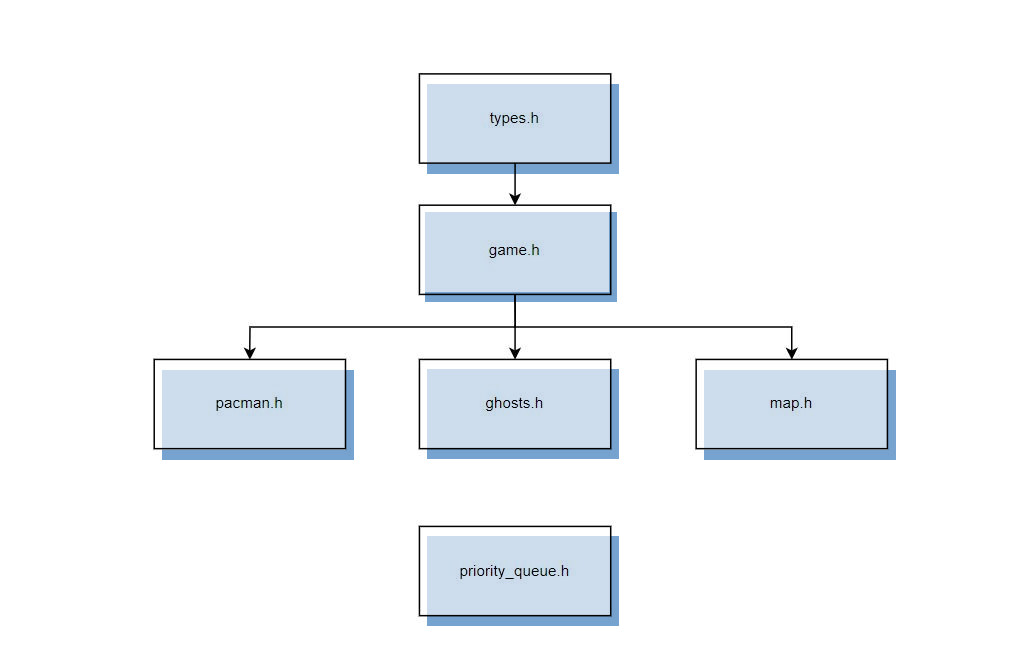
\includegraphics[scale=0.9]{pacman-overviewStylized.JPG}
\caption{An overview of the header files and their inter dependencies in the Pac-Man extension.}
\end{figure}


\subsection{Challenges}
The first challenge we faced was deciding on how we would implement the Pac-Man graphics. The two frameworks we considered using were SDL and Ncurses - we chose Ncurses due to its simplicity. During the beginning of the extension, we had little organisation and did not have the same planning stage as in the emulator and assembler – due to not being sure where to start. This caused the code to become convoluted and confusing to the point that we would have to search the entire project to find where constants were defined. This led to many bugs being introduced and painful debugging sessions. After two days, we decided to start again having an idea on what we would need to implement allowing us to follow the same procedure as in the emulator and assembler. We also found implementing the ghosts’ movements to be quite difficult. We implemented a targeting algorithm which allows each ghost to target specific areas based on the original game. We wanted to implement Dijkstra’s pathfinding algorithm. However, we did not manage to implement it correctly within the time frame.

\subsection{Testing} 
This was the first game many of us had made. We quickly discovered that unit tests are not as effective as simply implementing a feature and testing to see it works. We also would try to deliberately break the game and create segfaults (which will be shown in the presentation during the “Segfault Speed Run”). We started writing unit tests for collisions and movement of the characters. However, we soon discovered what we think will work ,theoretically, simply does not happen and there are many ways of breaking a game. Nevertheless, we did still create unit tests for the Priority Queue ADT used in the path finding algorithm.

\begin{figure}[h!]
\centering
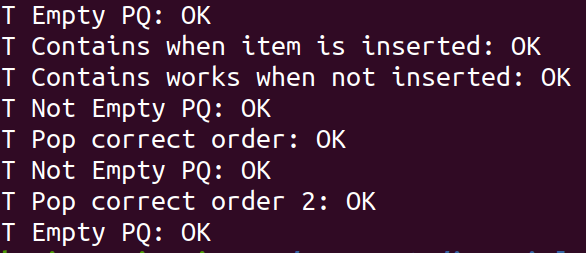
\includegraphics[scale=0.3]{priority_queue_test.png}
\caption{Unit Tests for Priority Queue ADT.}
\end{figure}

\section{Group Reflection}
\rule{\textwidth}{0.05em}
\vspace{0.1em}

Since for most of us this was the first time completing a group coding project, we had to learn how to use Git properly, split up the work based on each of our strengths and learn to debug each other’s code. As a team, we think we communicated well and managed to understand each other’s working timetables to maximise productivity.  Moreover, since we all live in North Acton Halls, this made collaboration easier as we were able to meet in person to plan out the project structure and clarify targets/deadlines we set for ourselves. When we were not able to meet in person, we would communicate via Teams and help each other over video calls, which - whilst helpful - was no substitute for in person meetings. \\ \par \noindent
Next time, we may choose to setup short daily/regular meetings to discuss where each of us are with our respective tasks and whether we need help from others/waiting on others to complete some of their code. This would help us understand the bottlenecks and whether we had to refocus our efforts on tasks, which were taking longer than expected. Next time, we think we should also take a ticket-based approach to completing tasks, where we breakdown the overall tasks into sequential sub-tasks (“tickets”), since in this project we worked concurrently on separate parts of the code, which may not be possible in future projects.


\section{Individual Reflection}
\rule{\textwidth}{0.05em}
\vspace{0.1em}

\subsection{Naman} 

This was my first extended group project and due to the current Covid situation, it has at times felt like a 4-person individual project. In this project, I felt it was a bit harder for me to collaborate since I was not in the same accommodation as my teammates and would have to write and debug my assigned parts individually. That said when we did meet to plan out the header files, we had a clear group strategy and targets. It was in these meetings I felt I was able to offer the most support, since I organised the header files clearly and helped make sure everyone knew what they were doing. My strengths lay in keeping on top of deadlines and communicating with the group regularly to establish progress. \\ \par \noindent
In terms of improvement for my next group project, I would like to be more flexible with my working hours. I prefer to work in the mornings, but I think that working at the same time as the rest of the group can be more productive as I am able to better support and collaborate with my group.


\subsection{Karim} 
This was my first large project in which I worked in a team to create specific programs. Although we dedicated time at the start to organise the structure and create header files, it was difficult to debug until others had completed their parts. This had the effect that we would think we had correctly implemented parts but once we merged the code, there would be a long process of debugging. \\ \par \noindent 
I feel that throughout the project, my main strength was my determination to continue working even when I was stuck with heavy debugging. Also, the ability to write modular code ensured that I was able to stick to the initial structure we agreed and write code that was easily debuggable. I feel I was flexible when it came to knowing that the current implementation was not working, and when to start again rather than trying to debug. This was particularly apparent when it came to the extension and after two days, myself and Konstantinos decided to create a new branch and start the implementation from the beginning. \\ \par \noindent
I feel that my main weakness, especially at the start, was not commenting my code when the implementation was not clear why I had chosen a specific way. Although this got better throughout the project, I feel that if I were to improve this next time, it would make it easier for my teammates to debug my code when I was not present to explain it.


\subsection{Konstantinos }
This was the first time I had to work in a group for such a big project. I found, especially in the beginning, we had a lot of trouble with merging our code and how to split the work evenly. There were a lot of times when people would finish their part and had to wait for others to finish and because of that we were quite late in finishing the emulator and assembler - meaning we did not have a lot of time to implement the extension. Also, we had people work on similar parts simultaneously causing there to be duplicated implementations at some points.\\ \par \noindent

 I want to believe that my flexible time schedule proved very useful in this project. I prefer to work in the morning but some other members prefer to work in the afternoon, so usually I would start coding in the morning and then meet with the other members in the afternoon and continue coding or help them with their parts. Therefore, I always had a good idea on what everyone was working on and could help anyone who was falling behind on their schedule. Also, especially in the assembler, I paid a lot of attention to the readability of my code, so it was one of the easiest parts to debug. Lastly, I believe my solutions to some of the problems we encountered were quite elegant. \\ \par \noindent

My main weakness was that I wrote too much code without testing, and that would sometimes create problems that would be easy to solve if the amount of code we had to look through was smaller. Also, mainly when coding in the evening my code became less idiomatic and I did not use many comments. Therefore, I had to waste time remembering how it functioned.\\ \par \noindent

For the next project, I believe each person should have a bigger part to implement so that two people do not have to solve similar problems. In addition, it is important to improve the clarity of our code so that maintenance will be less of a hassle.\\ \par \noindent


\subsection{Panayiotis}
Personally, I have worked on lots of group projects, some of which involved programming, before but none required the use of Git. Hence, I did not know how to properly use Git and I believe this would have been a major weakness on my part, if the rest of my teammates were used to collaborating with others via Git. I also expected the fact that I prefer to stay up late to work, and therefore wake up late, to present an obstacle to the team but it actually did not. This is because Karim and I both preferred this work style, while Konstantinos and Naman preferred working for the other half of the day so the two of them would work during the day and then we would take over for the night.\\ \par \noindent
If I were to list my strengths, one of them would be that I was quite flexible in the decisions we had to take us a group but at the same time I would provide the rest of the team with my views and opinions on a specific matter instead of just sitting back and waiting for them to decide. Moreover, I have always tried to write good comments on my code so that the others could easily read, understand, change, and debug it - if necessary. Last but not least, I believe that I was always verbose, in a good sense, about what I was working on, how it was going, and if I needed any help.\\ \par \noindent
For my next project, one thing I am definitely doing is discussing our working hours with the rest of the group. My usual approach to coding worked on this project, but it is not guaranteed to fit every other team I will have to work in.\\ \par \noindent

% \begin{figure}
% \centering
% \includegraphics[width=0.3\textwidth]{frog.jpg}
% \caption{\label{fig:frog}This frog was uploaded via the file-tree menu.}
% \end{figure}

\end{document}